\section{Using Digital Multimeters}
\label{digital_multimeters}

The diagrams below show the correct input jacks and settings to use 
for measuring DC voltages and currents 
with the black, BK 390 digital multimeters.

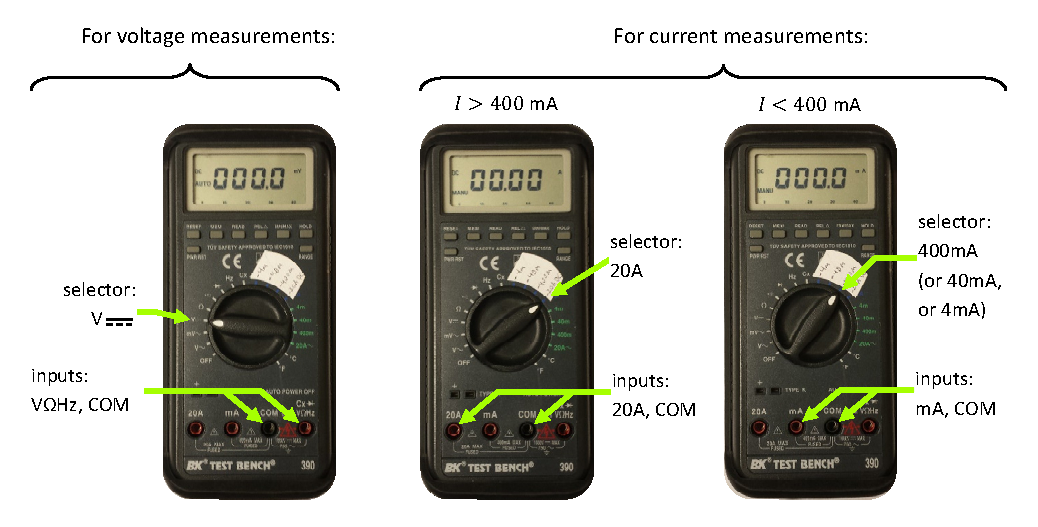
\includegraphics[width=\textwidth]{appendices/digital_multimeters/dmm_figs_bk390.eps}
\index{color_page}

\vspace{\fill}
For the red, Amprobe XR37 multimeters, the settings are very similar.

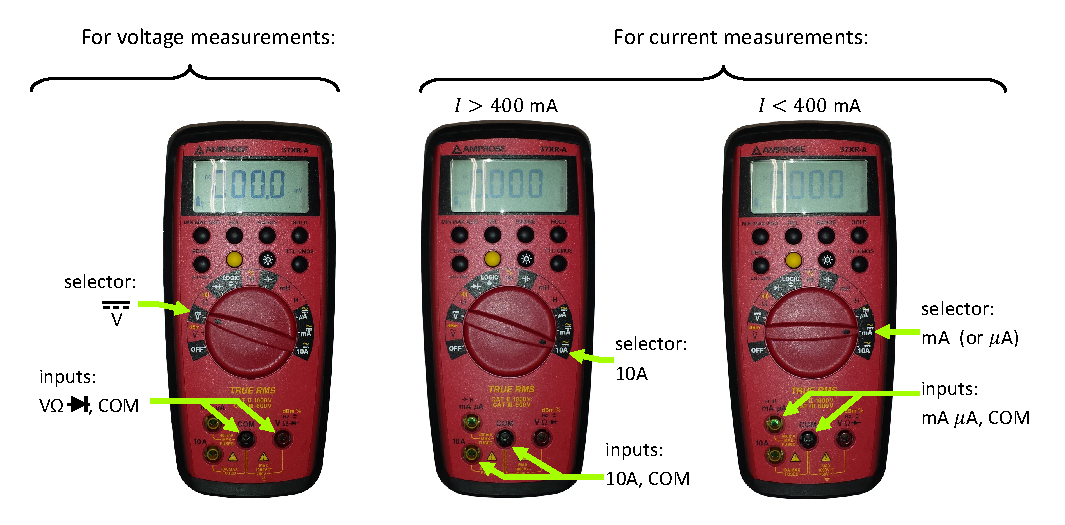
\includegraphics[width=\textwidth]{appendices/digital_multimeters/dmm_figs_xr37.eps}

\vspace{\fill}
When measuring currents, if you are unsure how large your current is, always start 
on the larger range (10A or 20A) and then decrease to mA or $\mu$A range if necessary.
Measuring a current larger than 400~mA on the mA ranges will cause you to blow a fuse in the multimeter.